\section{Results}
\label{section:experiments}

In this section, we introduce the metrics we define to measure performance, and we discuss some qualitative and quantitative results that give insights to our proposed \METHOD~method. 




\subsection{Metrics}
To evaluate accuracy of the layout estimation, we make use of geometric metrics applied between the ground-truth room layout and our predicted \METHOD~language. To do so, we define an \textit{entity distance}, $d_E$, between a pair of entities of the same class. Each entity, $E$, is represented as a 3D plane segment comprising of 4 corners $\{c_1, c_2, c_3, c_4\}$. The distance between two entities, $E$ and $E'$ is computed as the maximum Euclidean distance between each corner and its counterpart assigned via Hungarian mathcing, i.e.: $d_E(E, E') = \text{max}\{||c_i - c'_{\pi(i)}|| : i = 1, ..., 4\}$, where $\pi(i)$ is the permutation also found via Hungarian matching. 

We threshold $d_E$ to define the success criteria for the predicted entities. We compute the following metrics: 
\begin{itemize}
    % \item Mean Average Precision (mAP) -- each predicted entity is associated with a ground-truth entity through Hungarian matching. Average Precision (AP) is computed with order of retrieval determined by descending $d_E$ across a range of thresholds and averaged.
    \item F1 Score @ \textit{threshold} -- the F1 score of the set of predictions is computed at a single $d_E$ threshold.
    \item Average F1 Score -- the F1 score is computed across a range of entity distance thresholds and averaged.
\end{itemize}

The scores are computed for each class independently and averaged to overall score. In addition, scores are computed for each scene and averaged across the dataset. We use the following range of thresholds (cm) for the average F1 scores: $T = \{1, 2, ..., 9, 10, 15, 25, 30, 50, 75, 100\}$.


\begin{figure*}[t]
    \centering
    % 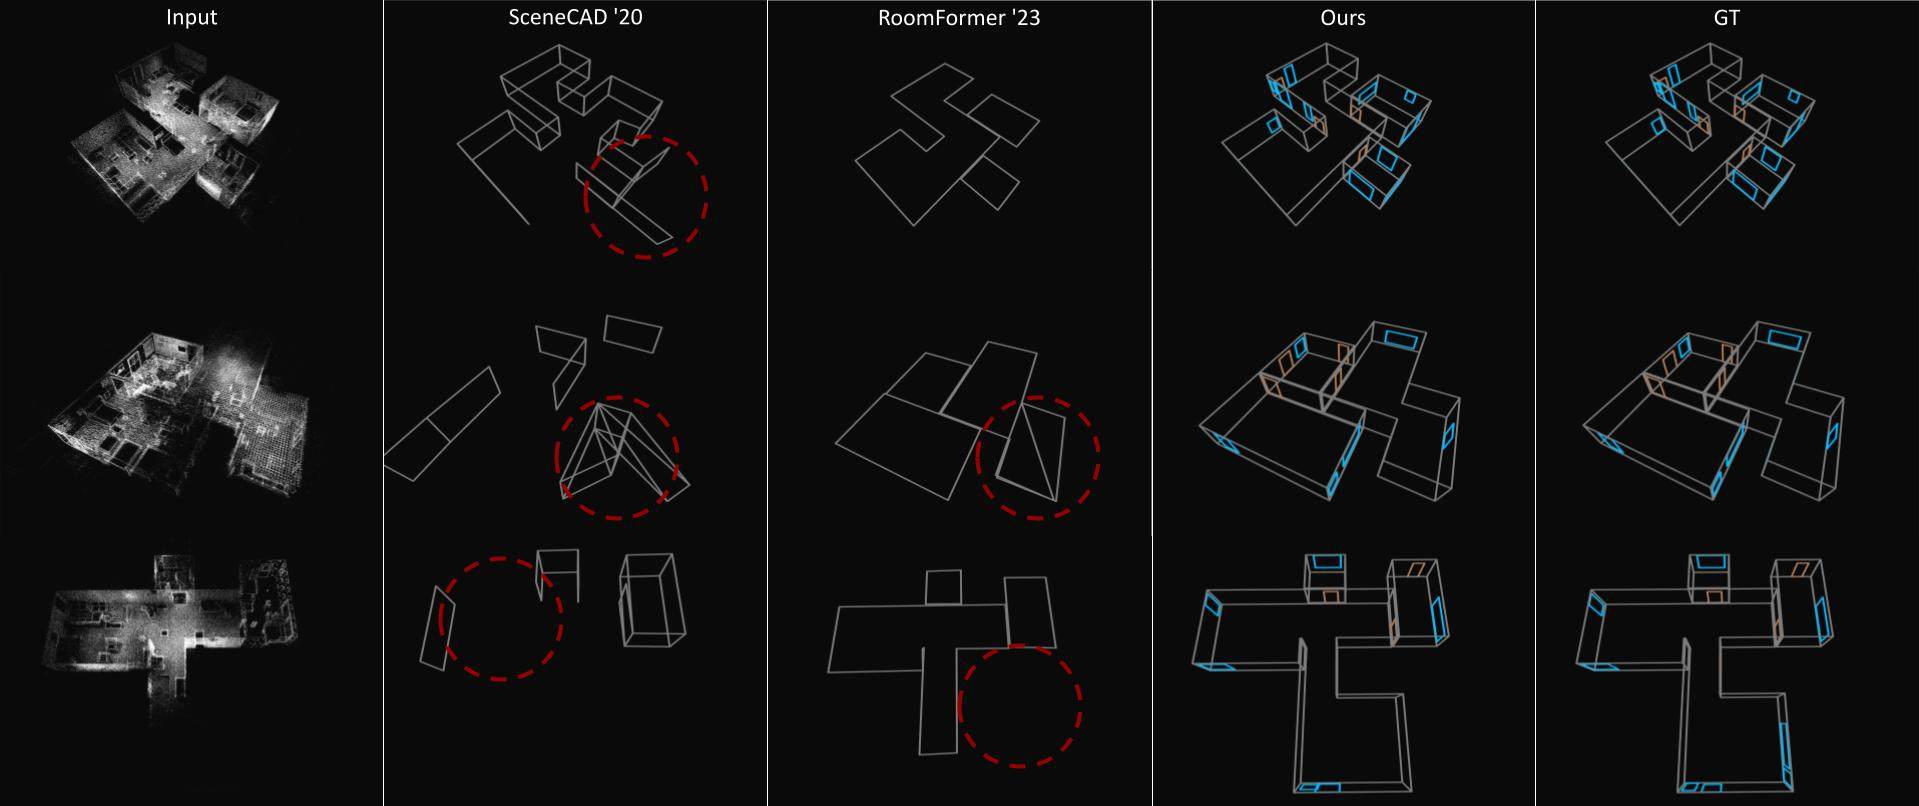
\includegraphics[width=\linewidth]{figs/qualitative_comparison_layout.jpg}
    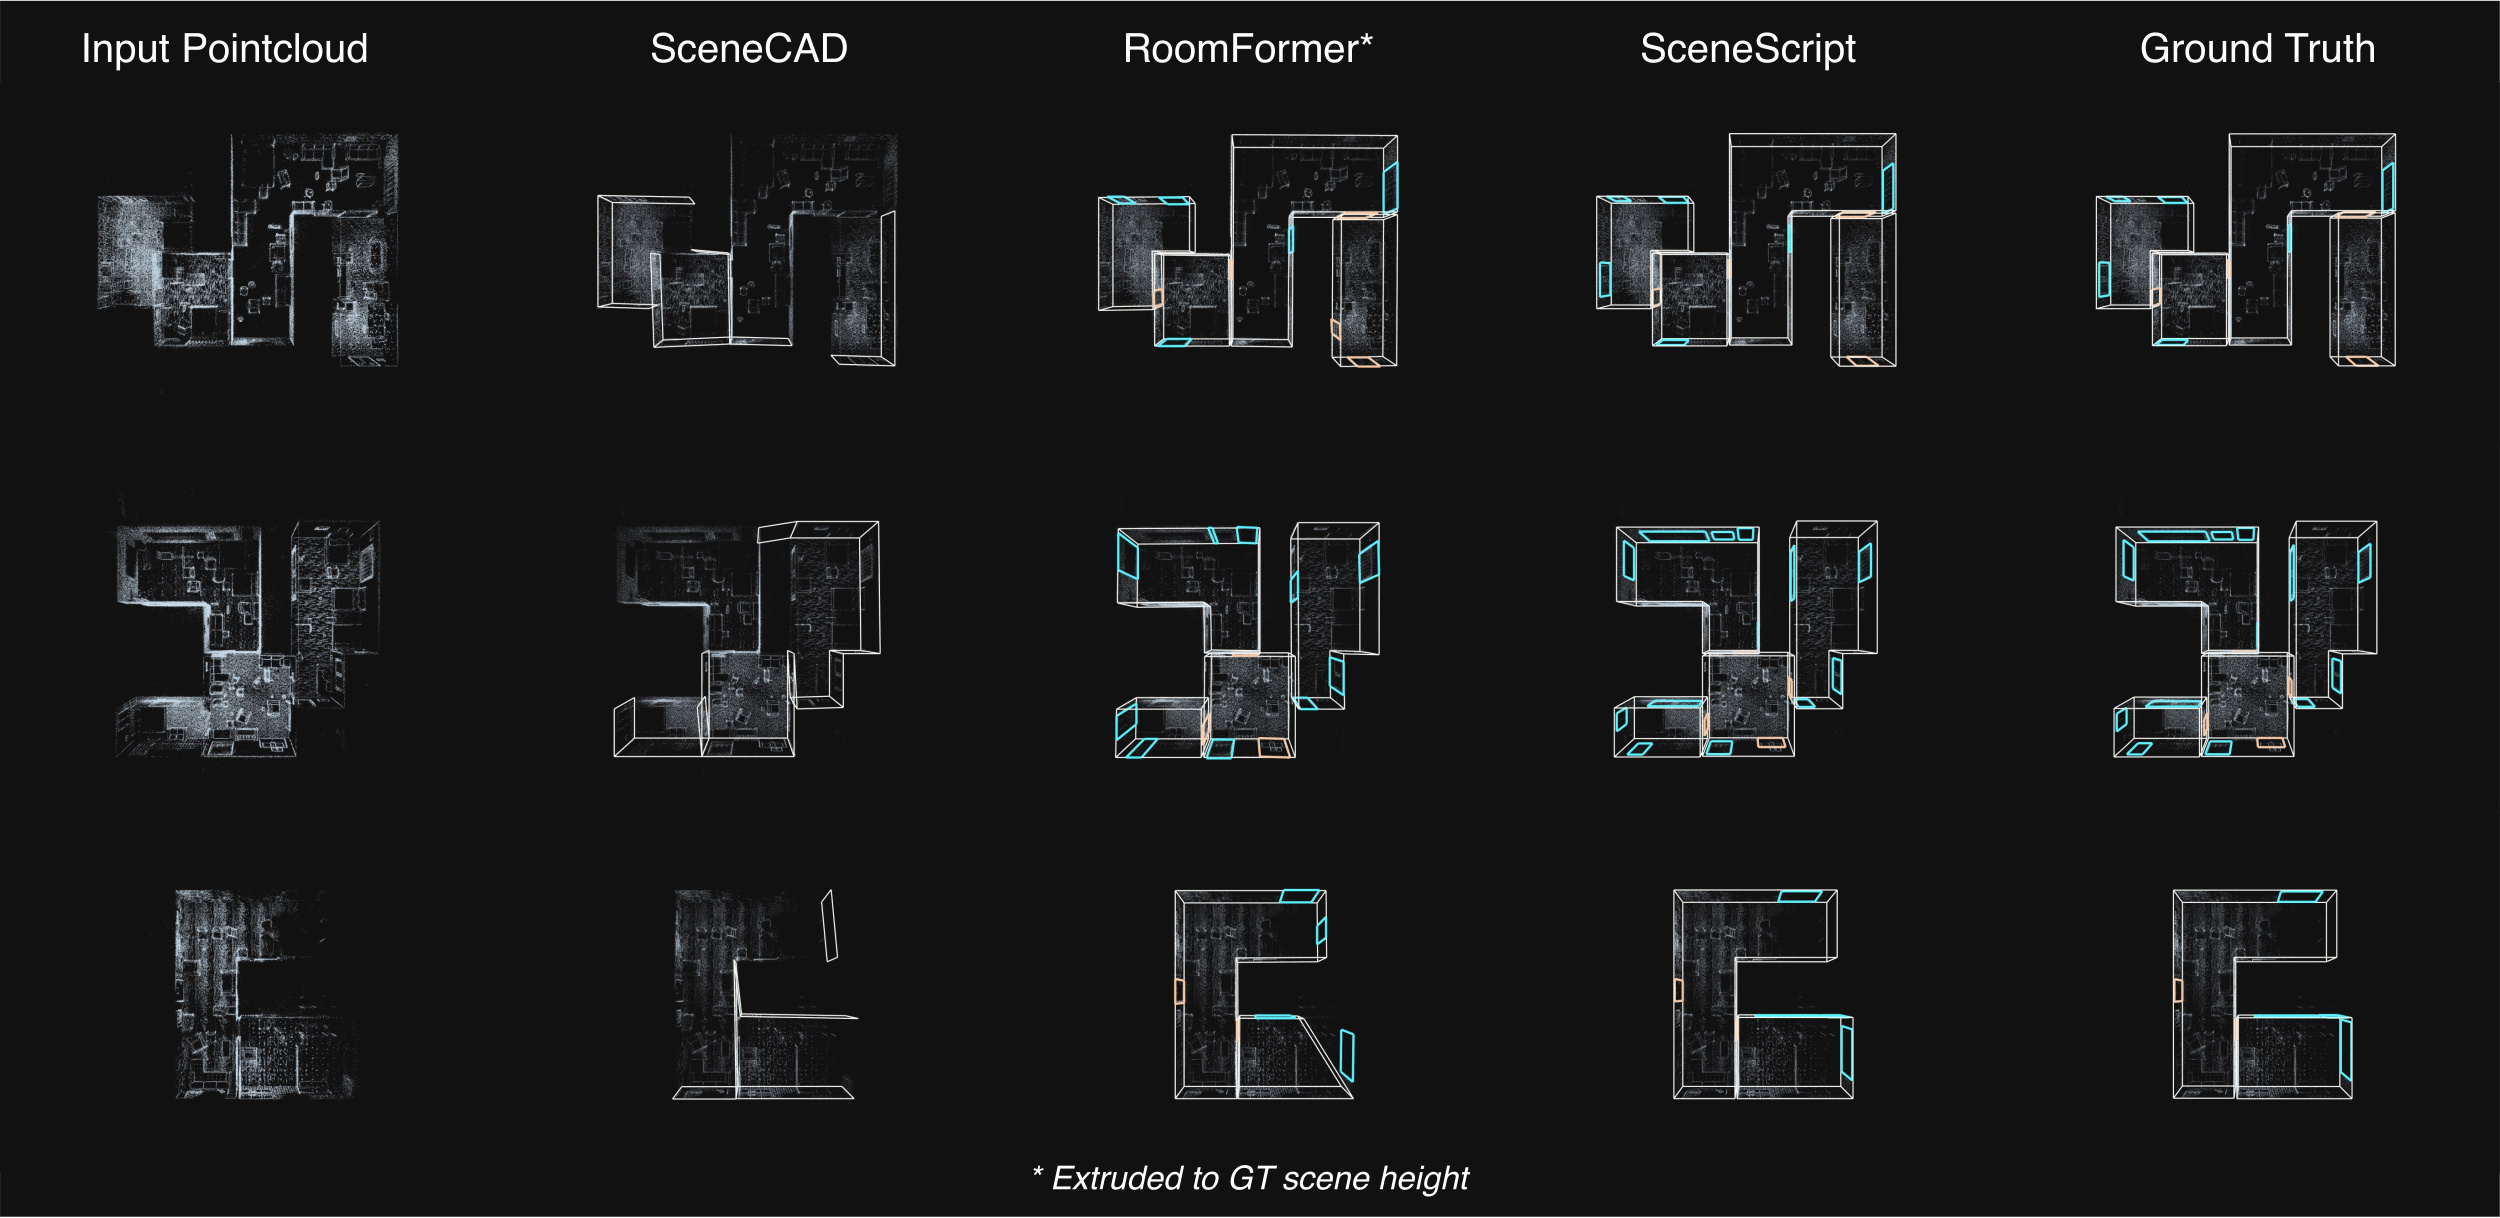
\includegraphics[width=\linewidth]{figs/layout_qualitative.jpg}
    \caption{Qualitative samples between our model and SOTA methods on \DatasetName's test set. Hierarchical methods like SceneCAD suffer from error cascading which leads to missing elements in the edge prediction module. RoomFormer (a 2D method extruded to 3D) primarily suffers from lightly captured scene regions which leave a unnoticeable signal in the density map. }
    \label{fig:qualitative_layout}
\end{figure*}

\subsection{Layout Estimation}


\begin{table*}[t]
    \centering
    \caption{\textbf{Layout Estimation on \DatasetName{}} Quantitative comparison between our method and related recent work. 
    % We can observe that our method significantly outperform previous work, across all metrics.
    % Recall that we compared only on wall predictions for fair comparison against all baselines.
    }
    % \resizebox{\textwidth}{!}{%
    \begin{tabular}{c|cccc|cccc}
         & \multicolumn{4}{c|}{F1 @5cm} & \multicolumn{4}{c}{Avg F1}\\
        Method & mean & wall & door & window & mean & wall & door & window \\
        \hline
        \hline
        SceneCAD '20~\cite{avetisyan2020scenecad}           & - & 0.048   & -  & -    & - & 0.275 & - & - \\
        % RoomFormer (orig) '23~\cite{yue2023connecting}      & 0.139 & 0.1 & - & -     & - & 0.120 & - & - \\
        RoomFormer '23~\cite{yue2023connecting}             & 0.139 & 0.159 & 0.148 & 0.110     & 0.464 & 0.505 & 0.481 & 0.407 \\
        \hline
        Ours (Point cloud)     & 0.848 & 0.930 & 0.922 & 0.692     & 0.784 & 0.816 & 0.811 & 0.724 \\
        Ours (Lifted features)  & \textbf{0.903} & \textbf{0.943} & \textbf{0.959} & \textbf{0.806}     & \textbf{0.801} & \textbf{0.818} & \textbf{0.822} & \textbf{0.764}\\
        Ours (Image-only)       & 0.661 & 0.687 & 0.798 & 0.497     & 0.719 & 0.727 & 0.772 & 0.658 \\

    \end{tabular}
    % }
    \label{tab:main_results_table}
\end{table*}



We perform scene layout estimation with the the three encoder variants of \METHOD: a baseline model with sparse3d convolution pointcloud encoder, an RGB RayTran-based feature volume encoder~\cite{tyszkiewicz2022raytran}, and our proposed lifted feature point encoder. The same transformer decoder is being used in all three scenarios. 
% The dataset is divided into training (100k scenes), and testing (1000 scenes) sets.

To provide comparison to existing works, we include results from two baseline methods, namely SceneCAD~\cite{avetisyan2020scenecad} and the recent  RoomFormer~\cite{yue2023connecting}. For these experiments SceneCAD and RoomFormer were both trained on \DatasetName. 
% We display results for both the pretrained RoomFormer, as well as a version finetuned on \DatasetName. 
Note that SceneCAD only predicts walls.
% While RoomFormer can predict doors/windows, we compared only on wall predictions for fair comparison against all baselines.
% See the supplement for baseline implementation details.

Table \ref{tab:main_results_table} shows the main results for our F1-based metrics on \DatasetName{}. \METHOD~exhibits a substantial performance advantage over SOTA layout estimation baselines across multiple metrics. 
% This strong performance is largely attributed to the effectiveness of our method in managing extremely high output resolutions. In contrast, RoomFormer is constrained by the coarse discretization of its 256-dimensional density map, while SceneCAD is limited by the coarse resolution of its heatmap voxel grid. 
Both baseline methods encounter a significant decline in accuracy when dealing with finer details. See Figure~\ref{fig:qualitative_layout} for qualitative comparisons between our method and baseline methods. 

% In Table~\ref{tab:s3d_results_table}, we further evaluate on the Structured3D dataset~\cite{Structured3D}. For this experiment, we configure \METHOD{} to use the same input as leveraged RoomFormer, \ie the scene pointcloud projected into a 2D density map, and predict a 2D equivalent of our previously defined commands. More details on this experimental setup will be included in the supplementary material. \todo{analyse results}

\subsubsection{Encoder Ablation.} 
The results demonstrate that \METHOD~is robust to the encoding strategy chosen to encode the egocentric capture. It is able to infer highly accurate scene layouts in all configurations tested, and in each case \METHOD~outperforms the included baselines by a significant margin. 

Relative comparison of the encoder strategies reveals that leveraging the pointclouds from a highly specialized and well-tuned system is still able to offer advantages of an, almost, entirely learned approach such as RayTran~\cite{tyszkiewicz2022raytran}. A light extension in the form of lifted image features can widen this gap even further. In particular, we observe that the discrepancy between the encoders becomes particularly apparent as the complexity of the scene increases in the form of increased room count -- more details are included in 
Appendix~\ref{app:num_rooms}.
% the supplementary material.
In Appendix~\ref{app:num_rooms}, we also show a quantitative evaluation 
% In the supplement, we also show a quantitative evaluation
of per-entity error distances, which aids in further attribution of relative performance gains between the encoding methods.
% This gives inspiration about future methods that might be able to combine both modalities in a more structured way in order to achieve even better results.



\begin{table}[t]
\centering
    \caption{\textbf{3D Object Detection} Performance comparison against state-of-the-art methods on an 3D object detection task trained and evaluated by F1-score at 0.25 and 0.5 IoU thresholds. By simply adding a \texttt{make\_bbox} command \METHOD{} can achieve competitive object detection results.
    }
    \begin{subtable}{0.48\linewidth}
    \centering
        \caption{\DatasetName}
        \resizebox{\textwidth}{!}{%
        \begin{tabular}{c|c|cc}
            & & \multicolumn{2}{c}{F1} \\
             Method & Input & @.25 IoU & @.50 IoU \\
            \hline \hline
            3DETR '21~\cite{misra2021end} & Points & 0.201 & 0.078 \\
            %SparseCNN~\cite{tang2022torchsparse} + 3DETR~\cite{misra2021end} & Points & 0.381 & 0.191 \\
            Cube R-CNN '23~\cite{brazil2023omni3d} & RGB &  0.394 & 0.228 \\
            ImVoxelNet '22~\cite{rukhovich2022imvoxelnet} & RGB & 0.584 & 0.516\\
            Ours & Points & \textbf{0.620} & \textbf{0.577} \\
        \end{tabular}
        }
        \label{tab:obj_det}
    \end{subtable}
    \begin{subtable}{0.48\linewidth}
    \centering
        \caption{ScanNet~\cite{dai2017scannet}}
        \resizebox{\textwidth}{!}{%
        \begin{tabular}{c|c|cc}
          & & \multicolumn{2}{c}{F1} \\
         Method & Input & @.25 IoU & @.50 IoU \\
         \hline \hline
         3DETR '21~\cite{misra2021end} & Points & 0.480 & 0.349\\
         3DETR-m '21~\cite{misra2021end} & Points & 0.536 & 0.407 \\
         SoftGroup '22~\cite{vu2022softgroup} & RGB Points & \textbf{0.622} & \textbf{0.573} \\
         Ours & RGB Points & 0.506 & 0.406 \\
        \end{tabular}
        }
        \label{tab:results_object_detection_scannet}
    \end{subtable}
\end{table}

\subsection{Object Detection}
In this section, we perform evaluation of \METHOD{} for object detection on both \DatasetName{} and ScanNet~\cite{dai2017scannet}. For comparison, we include recent and state-of-the-art baseline methods, namely Cube-RCNN~\cite{brazil2023omni3d}, ImVoxelNet~\cite{rukhovich2022imvoxelnet}, 3DETR~\cite{misra2021end}, and SoftGroup~\cite{vu2022softgroup}. 
% See the supplement for baseline details.
%If there are notable aspects, implementation details for these methods can be found in the supplementary material.

Worth noting is that \METHOD{} does not predict a confidence score for each \texttt{make\_bbox} command. This means that fair computation of the conventional mAP metric for this task is not possible, as detections cannot be ranked across scenes. Among other issues, this results in a metric that varies with the order in which scenes are evaluated. We therefore report F1-score-based metrics, which do not exhibit this order variance. Further discussion of this, and mAP numbers for the baselines for reference, can be found in 
% the supplementary material.
Appendix~\ref{app:baseline_map}.

% \subsubsection{Anonimized Dataset.}

%TODO: overall, our general purpose arch can hang with the big bois of objdet.
%In Tables~\ref{tab:obj_det} and~\ref{tab:results_object_detection_scannet}, \METHOD~demonstrates performance on par with SOTA baselines, indicating that learning to infer our proposed \METHOD~language representation does not suffer compared to specialised object detection network architectures.

In Table~\ref{tab:obj_det}, all methods were trained on \DatasetName. 
3DETR performs poorly due to its encoder being designed for relatively clean datasets such as ScanNet~\cite{dai2017scannet}, while semi-dense point clouds from \DatasetName{} exhibit more noise and less uniformity (see Figure~\ref{fig:main_pipeline} for an example).
Cube R-CNN and ImVoxelNet both operate on RGB images, and detections are tracked for the entire sequence via a tracker~\cite{brazil2023omni3d} to provide competitive performance. 
In Table~\ref{tab:results_object_detection_scannet}, our method provides similar performance to both 3DETR and SoftGroup.

Through the addition of the \texttt{make\_bbox} command, \METHOD~demonstrates object detection performance on par with SOTA baselines on multiple object detection datasets. 
This result illustrates the extensibility of a token-based approach, and that our proposed \METHOD~language representation does not suffer compared to specialised object detection network architectures.

